\chapter{Interazione radiazione-materia}
In questo capitolo ci occuperemo dell'interazione delle particelle con la materia, verrà diviso in tre sezioni : 
\begin{itemize}
        \item interazione di particelle cariche;
        \item interazione di fotoni; 
        \item interazione di neutroni.
\end{itemize}
\section{Interazione di particelle cariche con la materia}
Immaginiamo una particella con carica $\textit{z}e$ e massa m che attraversa un materiale di lunghezza $\dd{x}$ composto da atomi con numero di massa A e densità $\rho$
come in figura.
Ci chiadiamo quanto sia l'energia che perde la particella nell'attraversare il tratto $\dd{x}$ : 
\begin{align*}
    \frac{\dd{E}}{\dd{x}}
\end{align*}
\subsection{Perdita di energia per ionizzazione : la formula di Bohr}
Durante la derivazione della formula di Rutherford abbiamo assunto che se la particella ha un'interazione con il nucleo dell'atomo, la particella non perde 
energia siccome il nucleo ha una massa molto maggiore ma, così facendo, stiamo trascurando la possibilità di trasferire energia agli elettroni che è ciò che 
andremo a trattare in questa sezione.\\
\begin{figure}[!h]
    \centering
    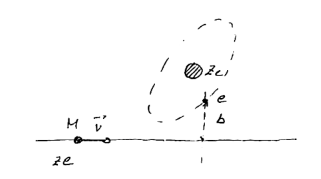
\includegraphics[scale=0.5]{ch6InterazioneMateria/BohrInterazione}
\end{figure}
\newpage
Dobbiamo calcolare l'energia cinetica ceduta all'elettrone ossia : 
\begin{align*}
        T_{e} = \frac{\Delta P_{e}^2}{2m_{e}}
\end{align*}
Per calcolare $\Delta P_{e}$ cambiamo sistema di riferimento in quello della particella dove quest'ultima è ferma e l'elettrone gli va incontro 
\begin{figure}[!h]
    \centering
    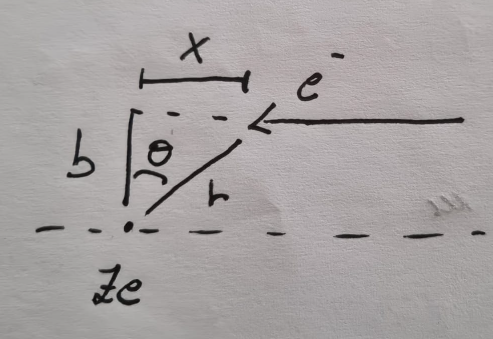
\includegraphics[scale=0.5]{ch6InterazioneMateria/CambioRiferimento}
\end{figure}

In una approssimazione non relativistica quindi possiamo vedere il tutto come un elettrone che passa nel campo culombiano di una particella con
carica $\textit{z}e$, attratto quindi da una forza : 
\begin{align*}
    F = \frac{\textit{z}e^2}{4\pi\epsilon_{0}}\frac{1}{r^2}
\end{align*}
possiamo dunque calcolare la quantità : 
\begin{align*}
        \Delta P_{e} &= \frac{\textit{z}e^2}{4\pi\epsilon_{0}}\int^{t}_{0}\frac{1}{r^2}\dd{t} \\
                     &= \frac{\textit{z}e^2}{4\pi\epsilon_{0}}\int^{\infty}_{-\infty}\frac{1}{r^2}\frac{\dd{x}}{v} \\
        \dd{t} &\rightarrow \frac{\dd{x}}{v} \tag*{Poichè v costante}
\end{align*}
Scomponiamo nelle due componenti considerando che $r = x^2 + b^2$ e che $(\Delta P)_{\parallel} = \Delta P\sin{\theta}$, $(\Delta P)_{\perp} = \Delta P\cos{\theta}$
otteniamo : 
\begin{align*}
        &(\Delta P)_{\parallel} =  \frac{\textit{z}e^2}{4\pi\epsilon_{0}v}\int\frac{1}{x^2 + b^2}\sin{\theta}\dd{x} = 0 \\
        &(\Delta P)_{\perp} =  \frac{\textit{z}e^2}{4\pi\epsilon_{0}v}\int\frac{1}{x^2 + b^2}\cos{\theta}\dd{x}
\end{align*}
\newpage
il secondo integrale lo calcoliamo sapendo che : 
\begin{align*}
        &\cos^2{\theta} = \frac{b^2}{x^2 + b^2} \\
        &\dd{x} = \frac{b}{\cos^2{\theta}}\dd{\theta}
\end{align*}
si ottiene : 
\begin{align*}
        (\Delta P)_{\perp} &=  \frac{\textit{z}e^2}{4\pi\epsilon_{0}vb}\int^{\frac{\pi}{2}}_{-\frac{\pi}{2}}\cos{\theta}\dd{\theta} \\
                           &= 2\frac{\textit{z}e^2}{4\pi\epsilon_{0}vb} \\
                           &= \frac{\textit{z}e^2}{4\pi\epsilon_{0}vb^2}\frac{2b}{v}
\end{align*}
\begin{tcolorbox}[colback=red!5!white,colframe=red!50!black,title=ATTENZIONE !]
nella formula sopra bisogna dire che : 
\begin{itemize}
        \item $ \frac{\textit{z}e^2}{4\pi\epsilon_{0}vb^2}$ = forza trasversale; 
        \item $\frac{2b}{v}$ = scattering time ; 
        \item abbiamo assunto che l'elettrone si muova su una linea dritta, ciò va bene se assumiamo che la velocità della particella sia molto maggiore 
                della velocità di orbita dell'elettrone.
\end{itemize}
\end{tcolorbox}
